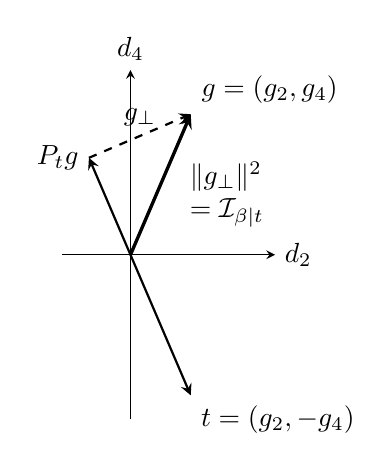
\begin{tikzpicture}[>=stealth,scale=2.55]
\draw[->] (-0.34,0) -- (0.72,0) node[right] {$d_2$};
\draw[->] (0,-0.82) -- (0,0.92) node[above] {$d_4$};
\coordinate (O) at (0,0);
\coordinate (G) at (0.30,0.70);
\coordinate (T) at (0.30,-0.70);
\coordinate (P) at (-0.2069,0.4828);
\draw[->,very thick] (O) -- (G) node[above right] {$\bm g=(g_2,g_4)$};
\draw[->,thick] (O) -- (T) node[below right] {$\bm t=(g_2,-g_4)$};
\draw[->,thick] (O) -- (P) node[left] {$P_t\bm g$};
\draw[->,thick,dashed] (P) -- (G) node[midway,above] {$\bm g_\perp$};
\node[align=left] at (0.48,0.30) {$\|\bm g_\perp\|^2$\\$=\mathcal I_{\beta\mid t}$};
\end{tikzpicture}
